\documentclass[tikz, border=5pt]{standalone}
\usepackage[dvipsnames]{xcolor}

\begin{document}
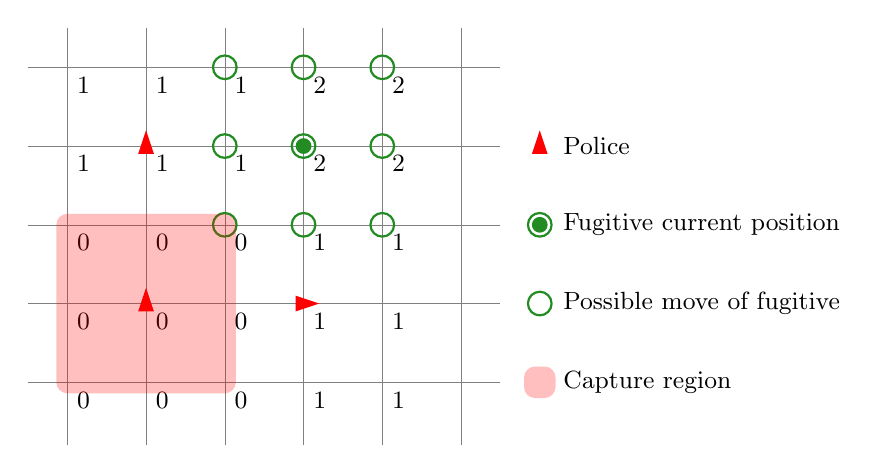
\begin{tikzpicture}

    %% Hamstrung squad game

    \newcommand{\policeUp}[2]{
        \fill[red] (#1,#2) -- ++(0,0.2) -- ++(0.1,-0.3) -- ++(-0.2,0) -- ++(0.1,0.3);
    }
    \newcommand{\policeRight}[2]{
        \fill[red] (#1,#2) -- ++(0.2,0) -- ++(-0.3,-0.1) -- ++(0,0.2) -- ++(0.3,-0.1);
    }
    \newcommand{\fugitive}[2]{
        \fill[ForestGreen] (#1,#2) circle (0.1);
    }
    \newcommand{\fugitiveHighlight}[2]{
        \draw[ForestGreen, thick] (#1,#2) circle (0.15);
    }

    \begin{scope}
        % Grid
        \draw[step=1cm,gray,very thin] (-0.5,-0.8) grid (5.5,4.5);

        % Labels
        \foreach \x in {0,1,2}
            \foreach \y in {0,1,2}
                \node[below right] at (\x,\y) {\small 0};
        \foreach \x in {0,1,2}
            \foreach \y in {3,4}
                \node[below right] at (\x,\y) {\small 1};
        \foreach \x in {3,4}
            \foreach \y in {0,1,2}
                \node[below right] at (\x,\y) {\small 1};
        \foreach \x in {3,4}
            \foreach \y in {3,4}
                \node[below right] at (\x,\y) {\small 2};

        % Players
        \policeUp{1}{1}
        \policeUp{1}{3}
        \policeRight{3}{1}
        \foreach \x in {2,3,4}
            \foreach \y in {2,3,4} {
                \fugitiveHighlight{\x}{\y}
            }
        \fugitive{3}{3}

        % Capture region
        \fill[red, rounded corners, opacity=0.25] (-0.14,-0.14) rectangle (2.14,2.14);
    \end{scope}

    % Legend
    \begin{scope}[xshift=6cm, yshift=3cm]
        \policeUp{0}{0}
        \node[right=5] at (0,0) {\small Police};
        \fugitive{0}{-1}
        \fugitiveHighlight{0}{-1}
        \node[right=5] at (0,-1) {\small Fugitive current position};
        \fugitiveHighlight{0}{-2}
        \node[right=5] at (0,-2) {\small Possible move of fugitive};
        \fill[red, rounded corners, opacity=0.25] (-0.2,-3.2) rectangle ++(0.4,0.4);
        \node[right=5] at (0,-3) {\small Capture region};
    \end{scope}

\end{tikzpicture}
\end{document}
